\documentclass[10pt,a4paper,onecolumn]{article}
% \usepackage[utf8]{inputenc}
\usepackage{marginnote}
\usepackage{graphicx}
\usepackage{xcolor}
\usepackage{authblk,etoolbox}
\usepackage{titlesec}
\usepackage{calc}
\usepackage{hyperref}
\hypersetup{breaklinks=true,
            bookmarks=true,
            pdfauthor=
{
      Mario Senden,
      Jannis Schuecker,,
      Jan Hahne,,
      Markus Diesmann,,
      Rainer Goebel,,
  },
            pdftitle=
{
[Re] A neural model of the saccade generator in the reticular formation
},
            colorlinks=true,
            citecolor=blue,
            urlcolor=blue,
            linkcolor=blue,
            pdfborder={0 0 0}}
\urlstyle{same}
\usepackage{tcolorbox}
\usepackage{ragged2e}
\usepackage{fontspec}
\usepackage{fontawesome}
\usepackage{caption}
\usepackage{listings}
\lstnewenvironment{code}{\lstset{language=Haskell,basicstyle=\small\ttfamily}}{}



%\usepackage{fancyvrb}
%\VerbatimFootnotes
%\usepackage{graphicx}
%\usepackage{mdframed}
%\newmdenv[backgroundcolor=lightgray]{Shaded}


\usepackage{longtable,booktabs}

\usepackage[
  backend=biber,
%  style=alphabetic,
%  citestyle=numeric
]{biblatex}
\bibliography{senden-schuecker-hahne-diesmann-goebel-2017.bib}



% --- Macros ------------------------------------------------------------------
\renewcommand*{\bibfont}{\small \sffamily}

\definecolor{red}{HTML}{CF232B}
\newcommand{\ReScience}{Re{\bfseries \textcolor{red}{Science}}}

\newtcolorbox{rebox}
   {colback=blue!5!white, colframe=blue!40!white,
     boxrule=0.5pt, arc=2pt, fonttitle=\sffamily\scshape\bfseries,
     left=6pt, right=20pt, top=6pt, bottom=6pt}

\newtcolorbox{repobox}
   {colback=red, colframe=red!75!black,
     boxrule=0.5pt, arc=2pt, left=6pt, right=6pt, top=3pt, bottom=3pt}

% fix for pandoc 1.14     
\newcommand{\tightlist}{%
  \setlength{\itemsep}{1pt}\setlength{\parskip}{0pt}\setlength{\parsep}{0pt}}

% --- Style -------------------------------------------------------------------
\renewcommand*{\bibfont}{\small \sffamily}
\renewcommand{\captionfont}{\small\sffamily}
\renewcommand{\captionlabelfont}{\bfseries}

\makeatletter
\renewcommand\@biblabel[1]{{\bf #1.}}
\makeatother

% --- Page layout -------------------------------------------------------------
\usepackage[top=3.5cm, bottom=3cm, right=1.5cm, left=1.5cm,
            headheight=2.2cm, reversemp, includemp, marginparwidth=4.5cm]{geometry}

% --- Section/SubSection/SubSubSection ----------------------------------------
\titleformat{\section}
  {\normalfont\sffamily\Large\bfseries}
  {}{0pt}{}
\titleformat{\subsection}
  {\normalfont\sffamily\large\bfseries}
  {}{0pt}{}
\titleformat{\subsubsection}
  {\normalfont\sffamily\bfseries}
  {}{0pt}{}
\titleformat*{\paragraph}
  {\sffamily\normalsize}


% --- Header / Footer ---------------------------------------------------------
\usepackage{fancyhdr}
\pagestyle{fancy}
%\renewcommand{\headrulewidth}{0.50pt}
\renewcommand{\headrulewidth}{0pt}
\fancyhead[L]{\hspace{-1cm}\includegraphics[width=4.0cm]{rescience-logo.pdf}}
\fancyhead[C]{}
\fancyhead[R]{} 
\renewcommand{\footrulewidth}{0.25pt}

\fancyfoot[L]{\hypersetup{urlcolor=red}
              \sffamily \ReScience~$\vert$
              \href{http://rescience.github.io}{rescience.github.io}
              \hypersetup{urlcolor=blue}}
\fancyfoot[C]{\sffamily \thepage}
\fancyfoot[R]{\sffamily Month 2017 $\vert$
                        Volume \textbf{1} $\vert$
                        Issue \textbf{1}}
\pagestyle{fancy}
\makeatletter
\let\ps@plain\ps@fancy
\fancyheadoffset[L]{4.5cm}
\fancyfootoffset[L]{4.5cm}

% --- Title / Authors ---------------------------------------------------------
% patch \maketitle so that it doesn't center
\patchcmd{\@maketitle}{center}{flushleft}{}{}
\patchcmd{\@maketitle}{center}{flushleft}{}{}
% patch \maketitle so that the font size for the title is normal
\patchcmd{\@maketitle}{\LARGE}{\LARGE\sffamily}{}{}
% patch the patch by authblk so that the author block is flush left
\def\maketitle{{%
  \renewenvironment{tabular}[2][]
    {\begin{flushleft}}
    {\end{flushleft}}
  \AB@maketitle}}
\makeatletter
\renewcommand\AB@affilsepx{ \protect\Affilfont}
%\renewcommand\AB@affilnote[1]{{\bfseries #1}\hspace{2pt}}
\renewcommand\AB@affilnote[1]{{\bfseries #1}\hspace{3pt}}
\makeatother
\renewcommand\Authfont{\sffamily\bfseries}
\renewcommand\Affilfont{\sffamily\small\mdseries}
\setlength{\affilsep}{1em}

\LetLtxMacro{\OldIncludegraphics}{\includegraphics}
\renewcommand{\includegraphics}[2][]{\OldIncludegraphics[width=12cm, #1]{#2}}


% --- Document ----------------------------------------------------------------
\title{[Re] A neural model of the saccade generator in the reticular formation}

    \usepackage{authblk}
                        \author[1, 2]{Mario Senden}
                    \author[3]{Jannis Schuecker,}
                    \author[4]{Jan Hahne,}
                    \author[3, 5, 6]{Markus Diesmann,}
                    \author[1, 2, 7]{Rainer Goebel,}
                            \affil[1]{Department of Cognitive Neuroscience, Faculty of Psychology and
Neuroscience, Maastricht University, 6201BC Maastricht, The Netherlands}
                    \affil[2]{Maastricht Brain Imaging Centre, Faculty of Psychology and Neuroscience,
Maastricht University, P.O. Box 616, 6200 MD Maastricht, The Netherlands}
                    \affil[3]{Institute of Neuroscience and Medicine (INM-6) and Institute for
Advanced Simulation (IAS-6) and JARA BRAIN Institute I, Jülich Research
Centre, 52428 Jülich, Germany}
                    \affil[4]{School of Mathematics and Natural Sciences, Bergische Universit"at
Wuppertal, Wuppertal, Germany}
                    \affil[5]{Department of Psychiatry, Psychotherapy and Psychosomatics, Medical
Faculty, RWTH Aachen University, 52062 Aachen, Germany}
                    \affil[6]{Department of Physics, Faculty 1, RWTH Aachen University, 52062 Aachen,
Germany}
                    \affil[7]{Department of Neuroimaging and Neuromodeling, Netherlands Institute for
Neuroscience, an Institute of the Royal Netherlands Academy of Arts and
Sciences (KNAW), 1105BA Amsterdam, The Netherlands}
            
\date{\vspace{-5mm}
      \sffamily \small \href{mailto:mario.senden@maastrichtuniversity.nl}{mario.senden@maastrichtuniversity.nl}}


\setlength\LTleft{0pt}
\setlength\LTright{0pt}


\begin{document}
\maketitle

\marginpar{
  %\hrule
  \sffamily\small
  %\vspace{2mm}
  {\bfseries Editor}\\
  Name Surname\\

  {\bfseries Reviewers}\\
        Name Surname\\
        Name Surname\\
  
  {\bfseries Received}  Month, Day, 2017\\
  {\bfseries Accepted}  Month, Day, 2017\\
  {\bfseries Published} Month, Day, 2017\\

  {\bfseries Licence}   \href{http://creativecommons.org/licenses/by/4.0/}{CC-BY}

  \begin{flushleft}
  {\bfseries Competing Interests:}\\
  The authors have declared that no competing interests exist.
  \end{flushleft}

  \hrule
  \vspace{3mm}

  \hypersetup{urlcolor=white}
  
    \vspace{-1mm}
  \begin{repobox}
    \bfseries\normalsize
      \href{http://github.com/rescience/rescience-submission/article}{\faGithubAlt~Article repository}
  \end{repobox}
      \vspace{-1mm}
  \begin{repobox}
    \bfseries\normalsize
      \href{http://github.com/rescience/rescience-submission/code}{\faGithubAlt~Code repository}
  \end{repobox}
        \hypersetup{urlcolor=blue}
}

\begin{rebox}
\sffamily {\bfseries A reference implementation of}
\small
\begin{flushleft}
\begin{itemize}
    \item[→] \emph{A neural model of the saccade generator in the reticular
formation}, G. Gancarz, S. Grossberg, Neural Networks, 1159-1174, 1998
  \end{itemize}\par
\end{flushleft}
\end{rebox}


\section{Introduction}\label{introduction}

We provide an implementation of the saccade generator (GM) model of the
neural circuitry in the reticular formation underlying saccadic eye
movements proposed by Gancarz \& Grossberg \autocite{Gancarz1998}. The
model forms part of (e.g.~is it an important paper in the domain ?). The
original implementation is not publicly available. T he implementation
we propose is coded in the NEST \autocite{Gewaltig2007} framework, one
of the modern actively developed simulation platforms that is publicly
available. The code uses the Python interface \autocite{Eppler2008} for
legibility. The model and analysis scripts are implemented using Python
2.7.12.

\section{Methods}\label{methods}

The methods section should explain how you replicated the original
results:

\begin{itemize}
\tightlist
\item
  did you use paper description
\item
  did you contact authors ?
\item
  did you use original sources ?
\item
  did you modify some parts ?
\item
  etc.
\end{itemize}

If relevevant in your domain, you should also provide a new standardized
description of the work.

\section{Results}\label{results}

Results should be compared with original results and you have to explain
why you think they are the same or why they may differ (qualitative
result vs quantitative result). Note that it is not necessary to redo
all the original analysis of the results.

\subsection{Saccadic staircase
simulation}\label{saccadic-staircase-simulation}

Bli Bla Blub

\begin{figure}
\centering
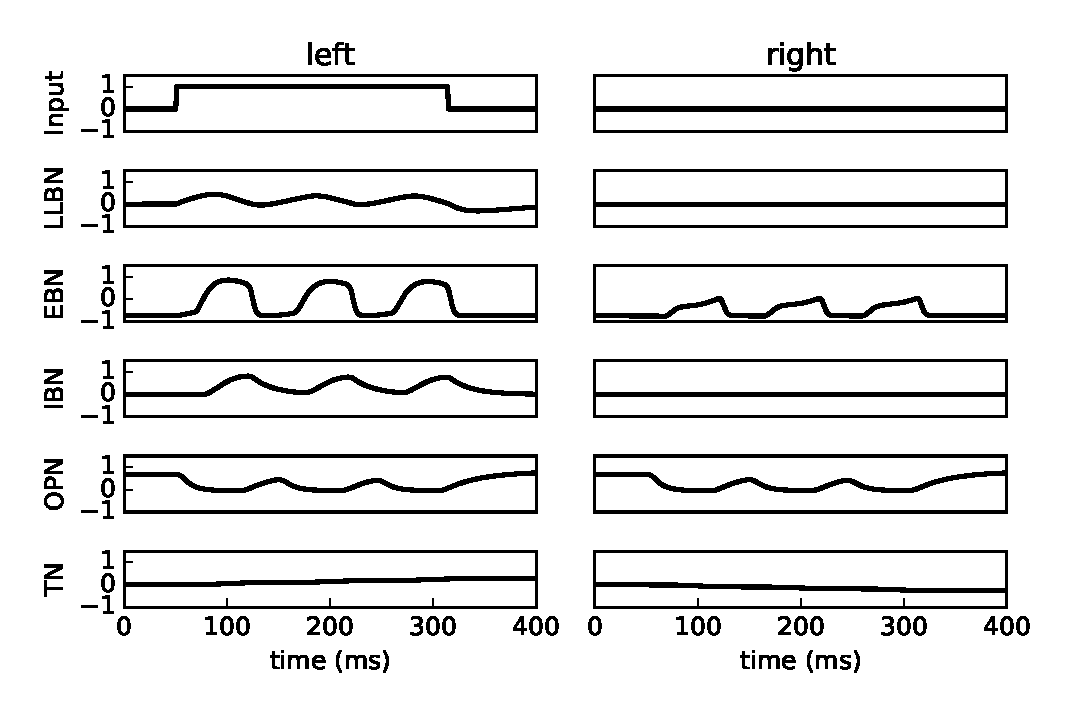
\includegraphics[width=11.60000cm,height=8.50000cm]{../code/fig3.eps}
\caption{\textbf{Figure caption for part (A) and part (B) .} Description
of stuff happening in the original implementation of Gancarz \&
Grossberg \autocite{Gancarz1998}.}\label{fig:fig_1}
\end{figure}

\subsection{Cell activity profiles in the reticular
formation}\label{cell-activity-profiles-in-the-reticular-formation}

Bli Bla Blub

\begin{figure}
\centering
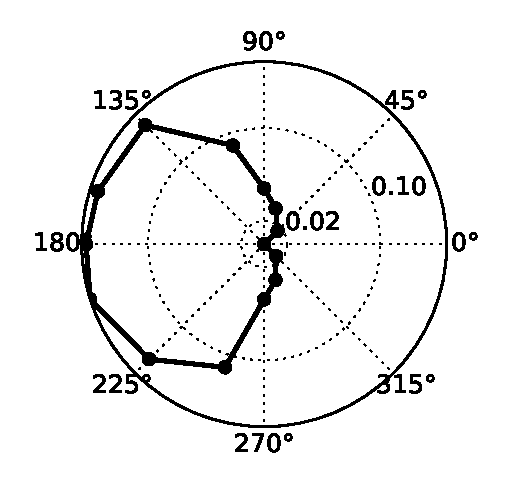
\includegraphics[width=8.50000cm,height=11.60000cm]{../code/fig5.eps}
\caption{\textbf{Figure caption for part (A) and part (B) .} Description
of stuff happening in the original implementation of Gancarz \&
Grossberg \autocite{Gancarz1998}.}\label{fig:fig_2}
\end{figure}

\subsection{Visually guided saccades}\label{visually-guided-saccades}

Bli Bla Blub

\begin{figure}
\centering
\includegraphics{../code/fig6.eps}
\caption{\textbf{Figure caption for part (A) and part (B) .} Description
of stuff happening in the original implementation of Gancarz \&
Grossberg \autocite{Gancarz1998}.}\label{fig:fig_3}
\end{figure}

\subsection{Oblique staircase
simulation}\label{oblique-staircase-simulation}

Bli Bla Blub

\begin{figure}
\centering
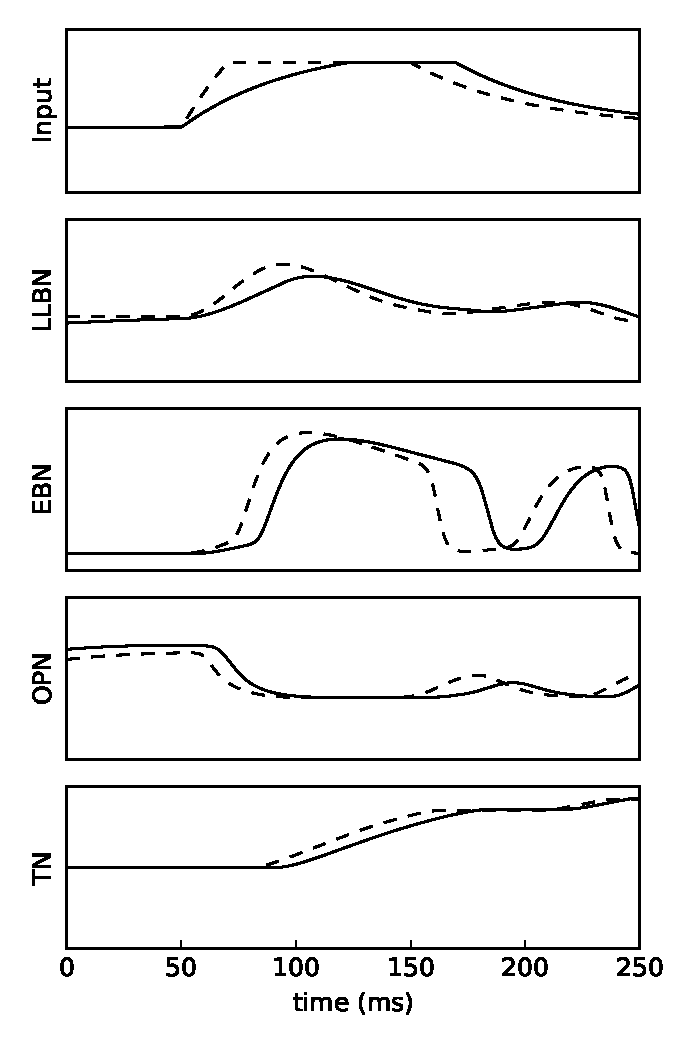
\includegraphics{../code/fig7.eps}
\caption{\textbf{Figure caption for part (A) and part (B) .} Description
of stuff happening in the original implementation of Gancarz \&
Grossberg \autocite{Gancarz1998}.}\label{fig:fig_4}
\end{figure}

\subsection{Tuning curve of excitatory burst neuron
(EBN)}\label{tuning-curve-of-excitatory-burst-neuron-ebn}

Bli Bla Blub

\begin{figure}
\centering
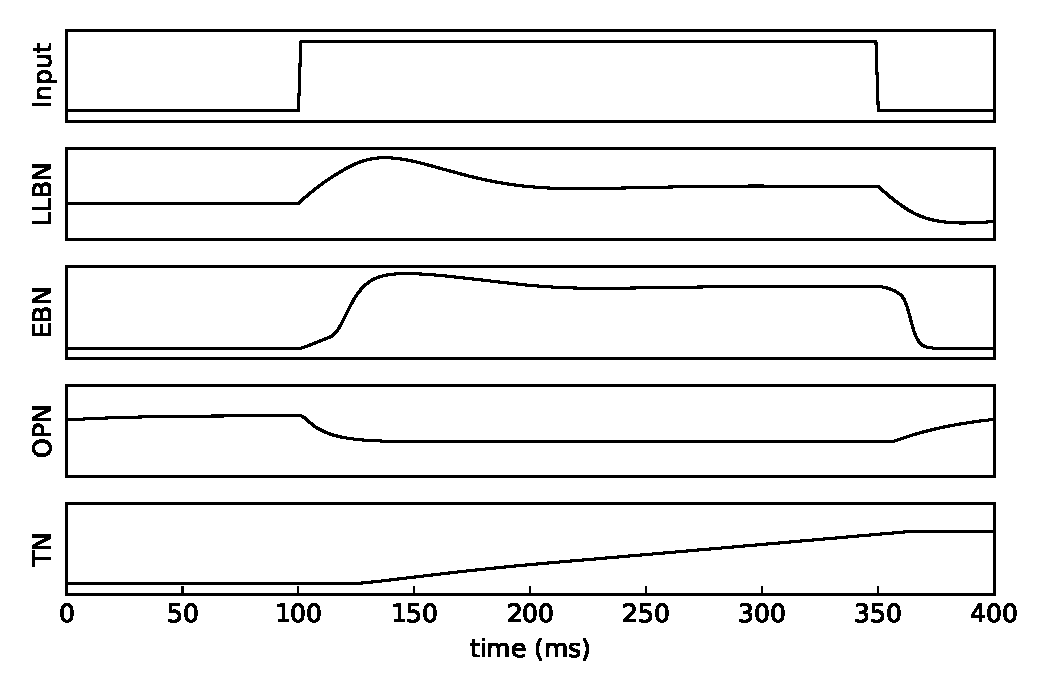
\includegraphics{../code/fig8.eps}
\caption{\textbf{Figure caption for part (A) and part (B) .} Description
of stuff happening in the original implementation of Gancarz \&
Grossberg \autocite{Gancarz1998}.}\label{fig:fig_5}
\end{figure}

\subsection{Effects of frequency of external
stimulation}\label{effects-of-frequency-of-external-stimulation}

Bli Bla Blub

\begin{figure}
\centering
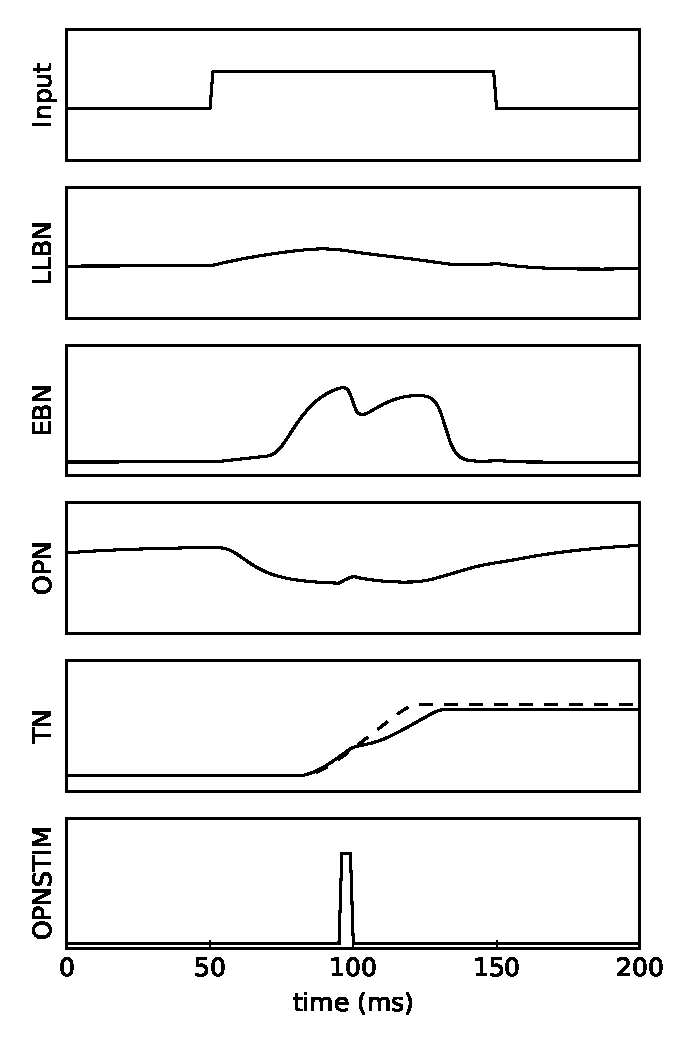
\includegraphics{../code/fig9.eps}
\caption{\textbf{Figure caption for part (A) and part (B) .} Description
of stuff happening in the original implementation of Gancarz \&
Grossberg \autocite{Gancarz1998}.}\label{fig:fig_6}
\end{figure}

\subsection{Trading saccade velocity and
duration}\label{trading-saccade-velocity-and-duration}

Bli Bla Blub

\begin{figure}
\centering
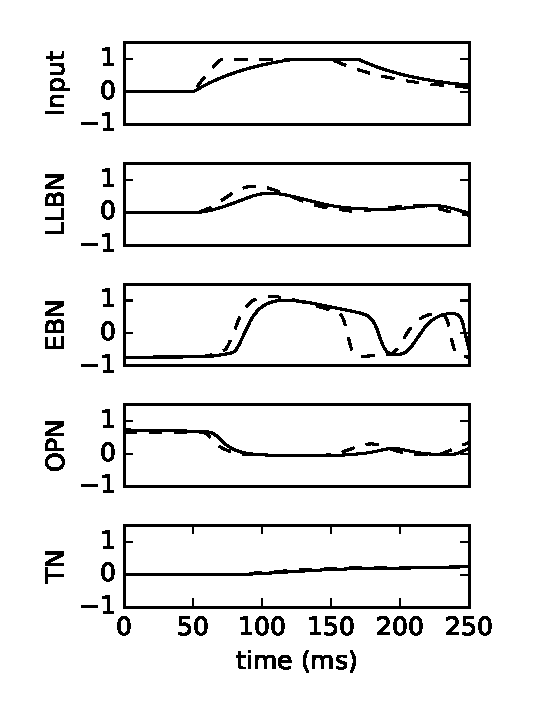
\includegraphics{../code/fig10.eps}
\caption{\textbf{Figure caption for part (A) and part (B) .} Description
of stuff happening in the original implementation of Gancarz \&
Grossberg \autocite{Gancarz1998}.}\label{fig:fig_7}
\end{figure}

\subsection{Smooth staircase
simulation}\label{smooth-staircase-simulation}

Bli Bla Blub

\begin{figure}
\centering
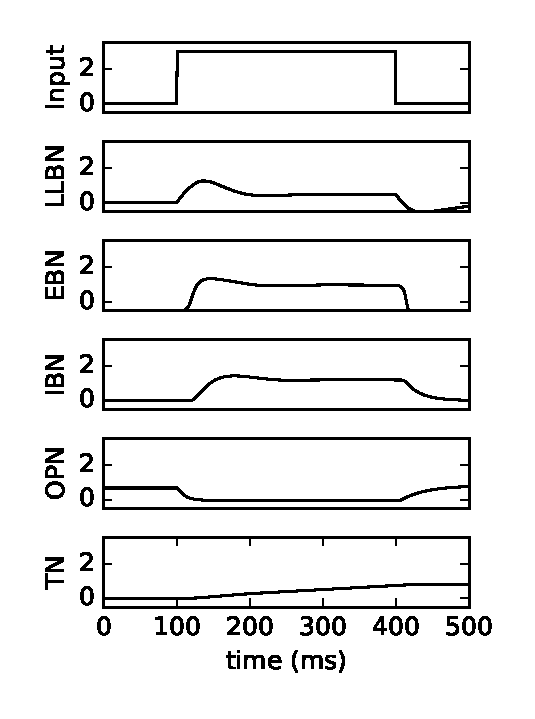
\includegraphics{../code/fig11.eps}
\caption{\textbf{Figure caption for part (A) and part (B) .} Description
of stuff happening in the original implementation of Gancarz \&
Grossberg \autocite{Gancarz1998}.}\label{fig:fig_8}
\end{figure}

\subsection{Interrupted saccade
simulation}\label{interrupted-saccade-simulation}

Bli Bla Blub

\begin{figure}
\centering
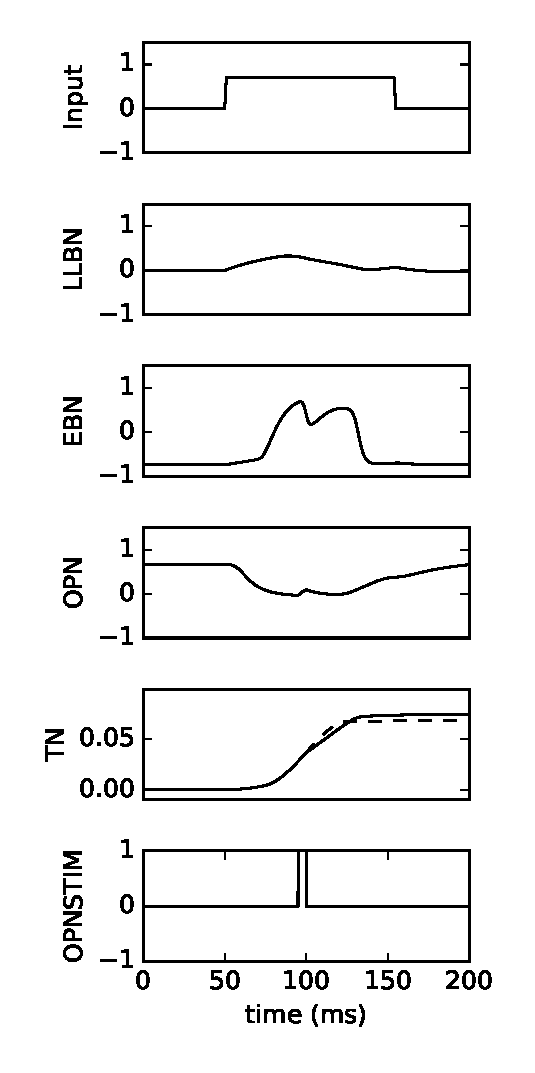
\includegraphics{../code/fig12.eps}
\caption{\textbf{Figure caption for part (A) and part (B) .} Description
of stuff happening in the original implementation of Gancarz \&
Grossberg \autocite{Gancarz1998}.}\label{fig:fig_9}
\end{figure}

\section{Conclusion}\label{conclusion}

Conclusion, at the very minimum, should indicate very clearly if you
were able to replicate original results. If it was not possible but you
found the reason why (error in the original results), you should exlain
it.

\begin{longtable}[]{@{}llllll@{}}
\caption{Table caption \{\#tbl:table\}}\tabularnewline
\toprule
Heading 1 & & & Heading 2 & &\tabularnewline
\midrule
\endfirsthead
\toprule
Heading 1 & & & Heading 2 & &\tabularnewline
\midrule
\endhead
cell1 row1 & cell2 row 1 & cell3 row 1 & cell4 row 1 & cell5 row 1 &
cell6 row 1\tabularnewline
cell1 row2 & cell2 row 2 & cell3 row 2 & cell4 row 2 & cell5 row 2 &
cell6 row 2\tabularnewline
cell1 row3 & cell2 row 3 & cell3 row 3 & cell4 row 3 & cell5 row 3 &
cell6 row 3\tabularnewline
\bottomrule
\end{longtable}

A reference to table \textcite{tbl:table}. A reference to figure
\textcite{fig:logo}. A reference to equation \textcite{eq:1}. A
reference to citation \textcite{markdown}.

\begin{figure}
\centering
\includegraphics{rescience-logo.pdf}
\caption{Figure caption}\label{fig:logo}
\end{figure}

\[ A = \sqrt{\frac{B}{C}} \] \{\#eq:1\}

\section{Acknowledgments}\label{acknowledgments}

All network simulations carried out with NEST
(http://www.nest-simulator.org).

{\sffamily \small
  \printbibliography[title=References]
}
\end{document}
